% \pagebreak
\section{Social Panoramas Using Wearable Computers}
\label{sec:pano}

A third example of annotation as interaction dimension on the Social AR Continuum is an annotation on 360-degree panoramic images. The level of annotation can be described as drawing or adding text, which then can be mapped into social proximity. This section discusses using panorama images to share social experiences. In particular, it explores awareness and annotation cues between users sharing a social experience through a shared panoramic image.

This work describes the concept of Social Panoramas that combine panorama images, Mixed Reality, and wearable computers to support remote collaboration \cite{Reichherzer2014, Billinghurst2014} (Figure \ref{fig:ismar14:concept}). A prototype was developed that allows panorama images to be explored in real-time between a Google Glass user and a remote tablet user. This uses a variety of cues for supporting awareness and enabling pointing and drawing. A user study was conducted to explore if these cues can increase Social Presence. The results suggest that increased interaction does not increase Social Presence, but tools with higher perceived usability show an improved sense of Presence.

\begin{figure}[ht]
    \centering
    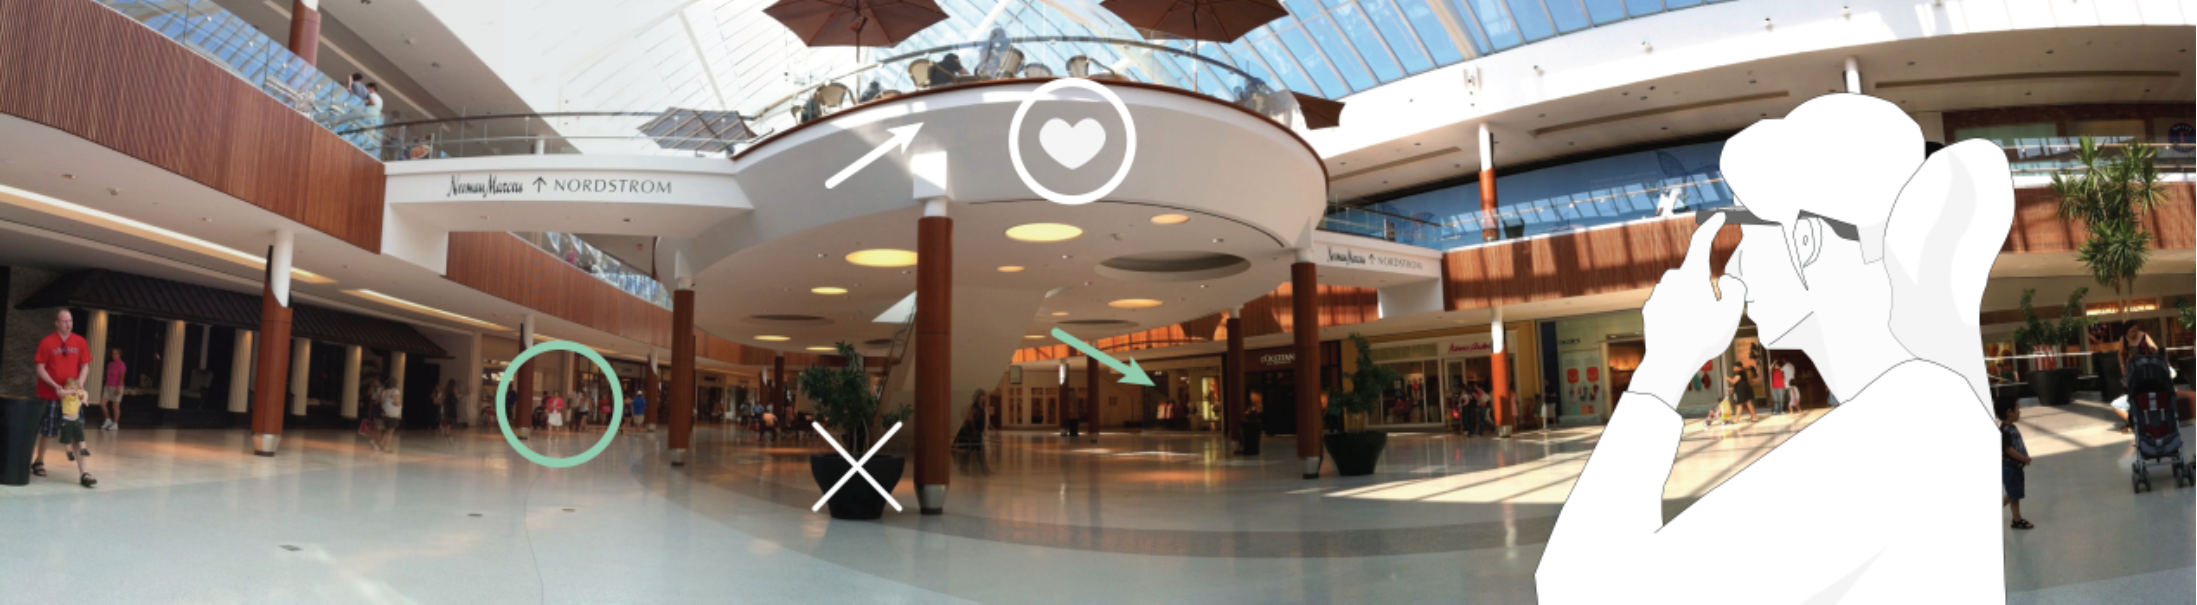
\includegraphics[width=\linewidth]{images/63-pano-ismar14/concept}
    \caption{Social Panoramas using Google Glass}
    \label{fig:ismar14:concept}
\end{figure}

Camera-equipped mobile devices provide a quick way of capturing and sharing experiences and spaces. Wearable computers that combine head-mounted displays (HMDs) and cameras provide new opportunities for collaboration. For example, Google Glass\footnote{http://www.google.com/glass/} has a camera, microphone, and head-worn display.

\subsection{Prototype Development}

In order to explore the concept of social panoramas, a prototype was developed that allowed a user with Google Glass to collaborate with a user on a tablet, both viewing and interacting with the same 360-degree panoramic image via a WiFi network. A Context Compass interface \cite{Suomela2000}  was implemented to provide awareness of the remote user's viewpoint. The prototype was developed using Processing \footnote{http://www.processing.org/} with the Ketai library for sensor support \footnote{https://code.google.com/p/ketai/} and the oscP5 networking library \footnote{http://www.sojamo.de/libraries/oscP5/}. The panorama was mapped onto a cylinder, viewed by the user rotating the tablet or their head with Glass. A within-subject experiment was conducted to compare if interaction possibilities such as drawing and pointing within a panorama can increase Social Presence, or "\textit{the sense of togetherness}" \cite{Basdogan2001}. 

The user interface (Figure \ref{fig:ismar14:pointing-drawing}) of the Glass and the tablet, shows the shared panoramic image in the background. To allow independent viewpoints between the two users, a Context Compass appears as a box on a line on top of the screen. It was designed to give overview information of the real world through head-mounted displays. The box moves accordingly to the head orientation on the line, which represents 360 degrees. The remote user is being displayed with a red box - once the rectangles are aligned, the users are looking at the same direction. The box moves only linearly.

The two users can interact with each other either using drawing or pointing. For the drawing interaction, the Glass users and tablet users alike could make use of drawing any shapes they like by utilising the touch surface of the tablet or the touchpad on the Glass device. Drawing would be done with one finger. Lifting a finger and touching again would result in a new shape being drawn. The pointing interaction is similar to the drawing interaction, but instead of drawing a continuous line only a pointer in the shape of an arrow would be visible and be used in the sense of pointing to objects or locations. The arrow would always be visible on-screen even if not in use.

\subsection{Experiment}

The experiment involved a collaborative task between two subjects in different rooms using Glass and Tablet devices, viewing the same panorama of the Glass user's environment. All subjects used four interaction conditions (Figure \ref{fig:ismar14:pointing-drawing}) that were counterbalanced with the technique of Latin square. The four conditions are:

\begin{itemize}
    \item C1-Audio: both participants used audio to communicate with each other and were able to see the panorama and the Context Compass, but they received no additional virtual cues. 
    \item C2-Pointing: a virtual pointer for each user was added that could be used as a cursor on the panorama.
    \item C3-Drawing: users could make use of the Glass touchpad or the touch surface on the tablet to draw on the panorama. 
    \item C4-Dual: this condition combined the Pointing and Drawing conditions; users were allowed to switch between them.
\end{itemize}{}

C2-Pointing and C3-Drawing were performed by using touchpad input on the side of Google Glass or touching the Tablet screen. After each trial, subjects filled out a Social Presence questionnaire consisting of eight questions on a seven-point Likert scale taken from Basdogan et al. \cite{Basdogan2001}. Usability was also measured with the System Usability Scale (SUS) \cite{brooke1996sus}.

\begin{figure}
    \centering
    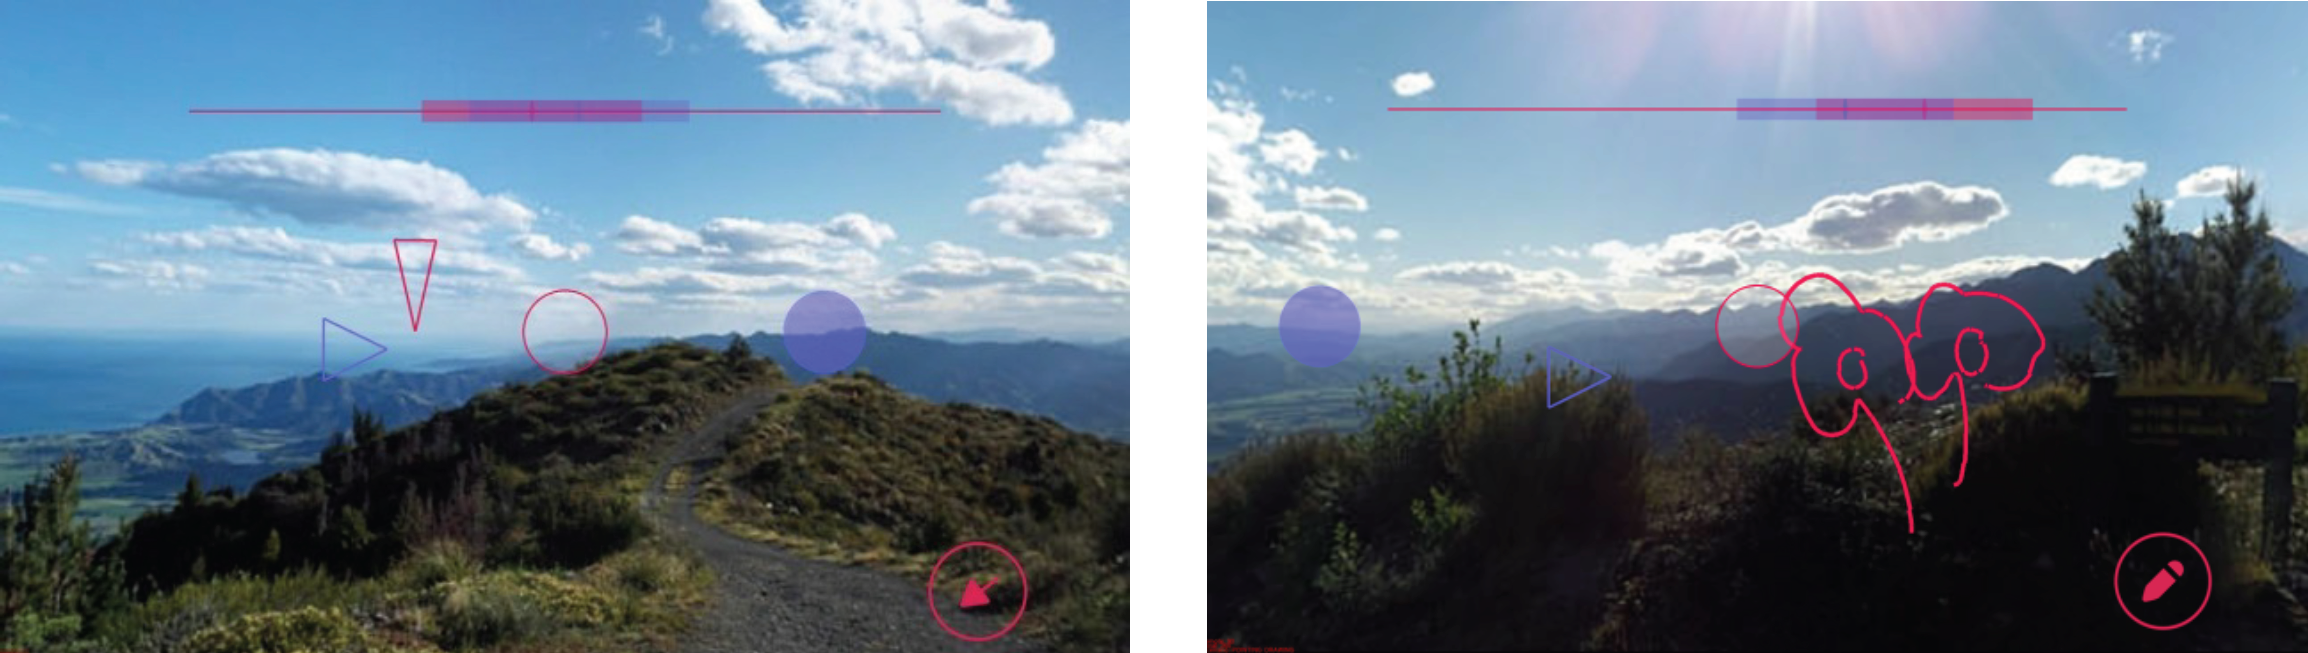
\includegraphics[width=\linewidth]{images/63-pano-ismar14/pointing-drawing}
    \caption{Triangular pointing cursor on the left, and drawing on the right. An icon indicates in which mode the user is.}
    \label{fig:ismar14:pointing-drawing}
\end{figure}

The subjects were given a list of furniture objects printed on a paper to describe to the other user the shape and discuss where to place this furniture item. Both of them could see the name of the object (e.g., "Mirror"), but only one could see the picture attached to it. The subject without the accompanying picture was asked to find a suitable place inside the panorama room (Figure \ref{fig:ismar14:envrionment-setup}), while the other would give a description and confirm or deny if the location was deemed realistic. Once both participants had agreed on a location, they would move on to the next object. They were given a maximum of three minutes. The Glass user was tasked to place objects in the room that they are in under guidance from the tablet person.

\begin{figure}
    \centering
    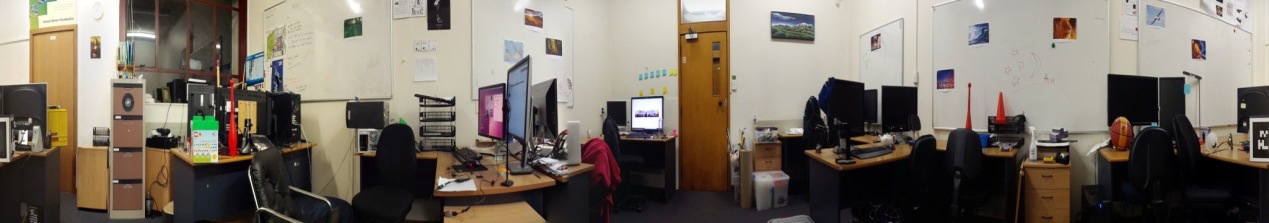
\includegraphics[width=\linewidth]{images/63-pano-ismar14/envrionment-setup}
    \caption{Panorama used for the study. The room represents the room of the Glass user.}
    \label{fig:ismar14:envrionment-setup}
\end{figure}

\subsection{Results}

There were 24 subjects aged between 18 and 45, divided into groups of two. Subjects did not know each other prior to the experiment and collaborated in pairs of their own gender to avoid any biases based on gender. Gender was equally distributed. Social Presence was measured as one single dimension. Figure \ref{fig:ismar14:social-presence} shows the overall Median values for each condition. The Drawing condition on Glass had a significantly lower Social Presence due to limited touch space on the Glass touchpad. 

The results of all eight questions of the Social Presence questionnaire were analysed with a Friedman test, which revealed a significant difference between the conditions for Glass users. ($\chi^2(3)=18.130, p<0.0005$). The significance level was set to p=0.0083 when a Bonferroni correction was applied. The following conditions were significantly different: Drawing-Audio ($Z=-3.794, p<0.0005$) and Drawing-Dual ($Z=-3.103, p=0.002$), resulting in Audio scoring the highest. There was no significant difference for tablet users.

\begin{figure}
    \centering
    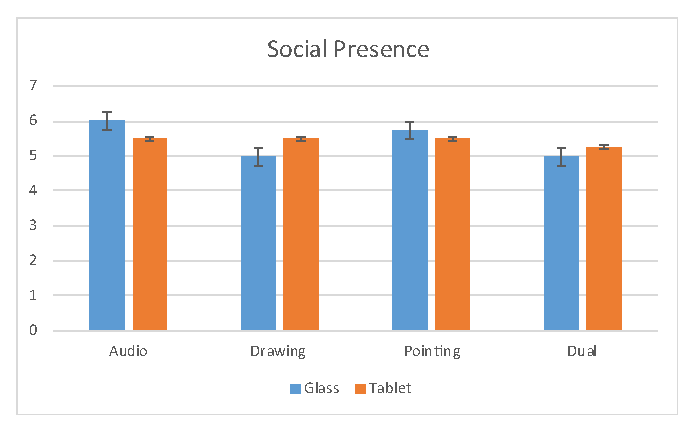
\includegraphics[width=.8\linewidth]{images/63-pano-ismar14/images-02.eps}
    \caption{Average results of social presence between glass and tablet}
    \label{fig:ismar14:social-presence}
\end{figure}

% \begin{table}[ht]
%     % Please add the following required packages to your document preamble:
%     % \usepackage{booktabs}
%     \caption{Median Social Presence values}
%     \centering
%     \begin{tabular}{@{}lllll@{}}
%     \toprule
%     \textbf{}       & \textbf{Audio} & \textbf{Drawing} & \textbf{Pointing} & \textbf{Dual} \\ \midrule
%     \textbf{Glass}  & 6              & 5                & 5.8               & 5             \\
%     \textbf{Tablet} & 5.5            & 5.5              & 5.5               & 5.3           \\ \bottomrule
%     \end{tabular}
%     \label{tbl:ismar14-results}
% \end{table}

The SUS survey (Figure \ref{fig:ismar14:sus}) was used to measure the usability of the interfaces, and both the Glass and tablet conditions were found to have good usability. The tablet Audio scored the highest with an average of $77.1\pm18.9$, which indicates a "good" usability \cite{Bangor2008}. Furthermore, the Drawing and Pointing conditions scored $70.4\pm21.4$ and $74.2\pm21.5$ respectively, also rated "good". However, the Dual condition scored merely $62.9\pm24$, reflecting the observation that users preferred to stay on one interaction tool during the Dual condition.

On Glass, the Audio usability was highest ($75.6\pm10.8$) followed by Pointing ($72.1\pm17.1$). The Dual mode was ranked as unacceptable ($58.1\pm18.6$) together with Drawing ($53.8\pm19.2$), showing the Glass touchpad was perceived as too difficult for drawing. A repeated-measures ANOVA determined that mean SUS scores differed statistically significantly between the conditions ($F(3, 33)=5,625025, P=0.003$) for Glass. There was a significant difference between Audio and the Drawing ($p<0.05$). A number of observations of user behaviour can be made. 
% Drawings were more commonly made to explain shape and dimensions, and pointing gestures were usually used to reference a location or an exact object. 

\begin{figure}
    \centering
    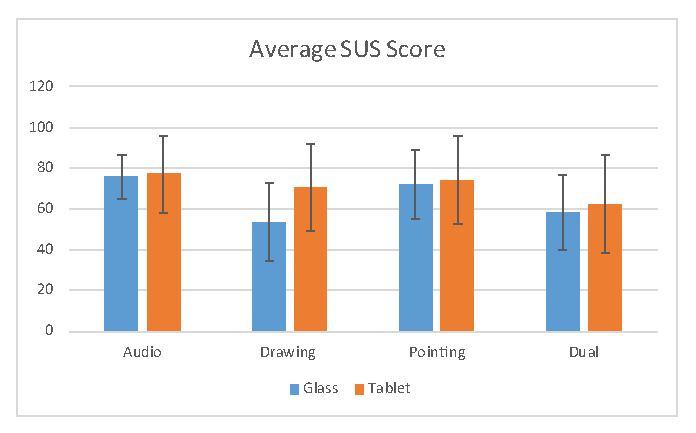
\includegraphics[width=.8\linewidth]{images/63-pano-ismar14/images-01.eps}
    \caption{Average results of SUS between glass and tablet}
    \label{fig:ismar14:sus}
\end{figure}

Tablet users generally preferred drawing to pointing and tried to draw the object shape (Figure \ref{fig:ismar14:tablet-drawing}). Due to difficulties with the touchpad, Glass users ended up using more abstract representations, such as rectangles or circles.

\begin{figure}
    \centering
    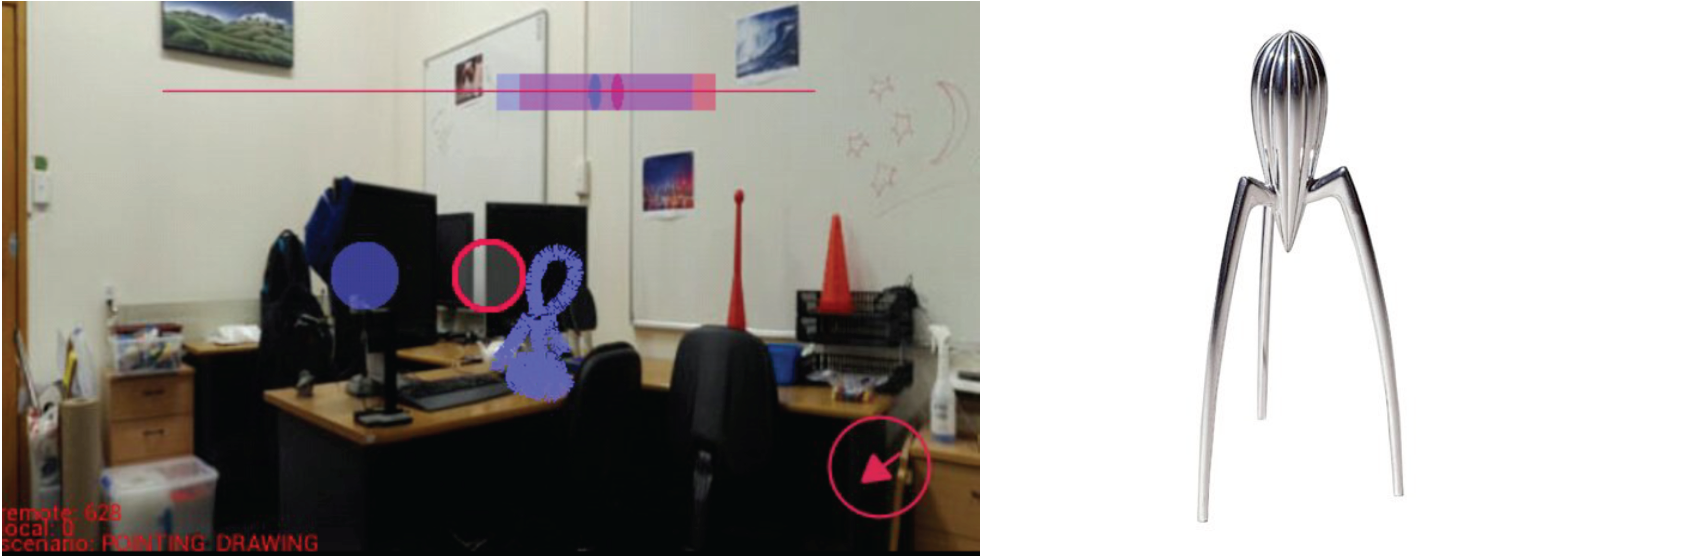
\includegraphics[width=\linewidth]{images/63-pano-ismar14/tablet-drawing}
    \caption{Tablet user attempting to draw an orange juicer}
    \label{fig:ismar14:tablet-drawing}
\end{figure}

\subsection{Observations}

Drawings were more commonly made to explain object shape and dimensions, and pointing gestures were usually used to reference a location or an exact object. Due to the limited space of touchpad on Glass, adding drawing and pointing options did not increase social presence.
% The Audio condition was the highest score in social Presence due to a lower level of interactivity between subjects and potential misunderstanding during the conversation when relying on Audio only to communicate. 

Local (Glass) users seemed to be engaged with the remote (Tablet) user by 1) following the orientation cues and being aware of their orientation comparing to the remote user's orientation, 2) being able to annotate (draw and point) on the image to improve their communication. The benefit of sharing panorama is to see the surrounding environment of the remote user, and have mirrored experiences.

This experiment found that adding interaction tools did not increase the Social Presence, compared to the Audio only interface. Users found drawing on the Glass touchpad difficult to use and ranked this as the worst condition for Social Presence, suggesting if a Social Panorama interface is not easy to use it will have a negative impact on Social Presence. 

% The results show that effective shared social experiences can be developed with panorama imagery, but more work still needs to be done. 

\subsection{Conclusions}

This section described the concept of Social Panoramas, using wearable computers, cameras and displays to share spaces in real-time. A prototype was developed on Google Glass and then used to explore the impact of interaction on Social Presence in a user study. 

Results found a difference in Social Presence between the Audio only condition and those that involved drawing interaction on Glass. Similarly, Audio scored the highest on Glass for usability compared to the Drawing and Dual condition. There was a clear preference from users for pointing tools. However, drawing on the Glass touchpad was perceived as difficult. These results show that effective, shared social experiences can be developed with panorama imagery, but more work still needs to be done.
Despite adding higher fidelity of annotation (drawing or pointing), in this specific platform (Glass), it did not lead to higher social presence. This indicates that the platform capability can play a factor in social presence in addition to the level of fidelity of the interaction method.


% In the future, there are a number of ways that this research could be extended. First, we could explore ways to overcome the drawing problem on Glass, such as using predefined simple geometric shapes such as circles and rectangles that could be observed being drawn during the experiment. Another possibility for future work is to offer a live-stream of the current field of view of the local user, enabling the Mixed Reality view to show a combination of the captured image and live video. These new interface elements will have to be evaluated in a further series of experiments focusing on usability and Social Presence.

